\documentclass{ieeeaccess}
\usepackage[utf8]{inputenc}
\usepackage[T1]{fontenc}
\usepackage{cite}
\usepackage{amsmath,amssymb,amsfonts}
\usepackage{amsthm}
\usepackage{algorithm}
\usepackage{algorithmic}
\usepackage{graphicx}
\usepackage{textcomp}
\usepackage{subfigure}
\usepackage{color}
\usepackage{rotfloat}
\usepackage{tabularx}
\usepackage{multirow}
\usepackage{float}
\usepackage[para]{threeparttable}
\renewcommand{\algorithmicrequire}{\textbf{Input:}}
\renewcommand{\algorithmicensure}{\textbf{Output:}}
\usepackage{bm}
\usepackage{booktabs}
\newcommand{\tabincell}[2]{\begin{tabular}[t]{@{}#1@{}}#2\end{tabular}}
\theoremstyle{definition}
\newtheorem{defn}{Definition}
\newcolumntype{C}{>{\centering\arraybackslash}X} % centered version of "X" type
\setlength{\extrarowheight}{1pt}

\def\BibTeX{{\rm B\kern-.05em{\sc i\kern-.025em b}\kern-.08em
    T\kern-.1667em\lower.7ex\hbox{E}\kern-.125emX}}

% This command is used to modify the paper. After the paper is definive. Please comment or delete this command.
\newcommand{\change}[2]{\textcolor{red}{#1}\textcolor{blue}{#2}}

\begin{document}
\history{Date of publication xxxx 00, 0000, date of current version xxxx 00, 0000.}
\doi{10.1109/ACCESS.2017.DOI}

\title{CBFS: A Clustering-Based Feature Selection Mechanism for Network Anomaly Detection}
\author{
    \uppercase{Jiewen Mao},
    \uppercase{Yongquan Hu},
    \uppercase{Dong Jiang},
    \uppercase{Tongquan Wei},\IEEEmembership{Senior Member, IEEE}, \uppercase{Fuke Shen}}
\address{School of Computer Science and Technology, East China Normal University, Shanghai 200062, China}

\markboth
{J. Mao \headeretal: CBFS: A Clustering-Based Feature Selection Mechanism for Network Anomaly Detection}
{J. Mao \headeretal: CBFS: A Clustering-Based Feature Selection Mechanism for Network Anomaly Detection}

\corresp{Corresponding author: Tongquan Wei (e-mail: tqwei@cs.ecnu.edu.cn).}

\begin{abstract}
Network traffic flows contain a large number of correlated and redundant features, which may significantly reduces the performance of data-driven network anomaly detection.
In this paper, we propose a novel clustering-and-ranking-based feature selection mechanism to reduce redundant features in network traffic, which can greatly improve the efficiency and accuracy of feature-based network anomaly detection. 
First, our proposed mechanism calculates the distance between feature vectors, merges them into different clusters, and selects the center of each cluster as a representative.
Second, the proposed mechanism integrates the information gain and gain rate of features to further streamline the number of features on the basis of clustering generation.
Third, we apply the decision-tree-based classifier to the generated subset of features, and finally detect the abnormal traffic flows.
The experimental results show that our proposed mechanism is effective in reducing their dimensions across different datasets, with feature reduction rates able to reach 20\% to 70\%. Network anomaly detection can achieve better cost-performace using a subset of features selected by our proposed mechanism. Compared to the benchmark method, our method can improve the cost-performance ratio by up to 70\% or more.
\end{abstract}

\begin{keywords}
    feature selection, clustering, information gain, classification, decision tree, intrusion detection
\end{keywords}

\titlepgskip=-15pt

\maketitle

% \tableofcontents

\section{Introduction}
\label{sec:introduction}

\PARstart{T}{he} daily network traffic of global users is predicted to more than 200 EB per month \cite{cisco-report} with the development of new technologies such as the Internet of Things and 5G mobile networks. 
At the same time, the amount of abnormal traffic growth in the network is also increasing. 
In order to detect abnormal network traffic more efficiently and accurately, machine learning and data mining algorithms are used to extract, analyze, and find the patterns of traffic data, build the models to adapt the data and classify every flow. 
However, These abnormal flows have the characteristics of both high quantity and high dimension. This may cause problems for classification results, such as over-fitting, high computational cost, and long training time. In order to improve the performance of classifiers, the features with high importance should be selected.

Generally, feature selection methods contains three types: filter, wrapper and embedded \cite{Maza2018, Cai2018}. Filter approach uses the statistical learning data as a measure to evaluate the attributes independently of classification algorithm\cite{Maza2018}. Hajisalem \emph{et~al.} \cite{Hajisalem2018} use correlation-based feature selection in their proposed IDS method. However it only selects the features related to targets. 
Wrapper approach uses the classification algorithms to select the best features. It uses accuracy (or area under curve, i.e. AUC) as a feedback to determine the effectiveness of feature subsets. A classical wrapper method is recusive feature elimination (RFE) \cite{RFE2002}. It eliminates features recursively until the classifier performs best on the remaining subset of features. 
Embedded methods allow the classifier perform training and feature selection simultaneously, and the classifier is allowed to decide the features to use. Typical tree-based classifiers involve the feature selection process, including decision tree (DT) \cite{quinlan2014c4}, random forest (RF)\cite{rf2002}, gradient boosting trees (GBDT) \cite{gbdt2001}, etc. Importances of features can be obtained after the classification is complete.

Existing feature selection methods mainly focus on the relationship between features and labels. 
However, in network data sets, one feature may have correlations with other features. 
These correlated features may also be selected by traditional feature selection methods, and the classifier may accept redundant features, which may result in low classifying accuracy. 
In addition, in theory, the optimal feature subset can be obtained by RFE (i.e. the feature subset that allows the classifier to achieve the highest performance), but in high-dimensional data, the time cost of RFE is unacceptable for practical engineering. 
Therefore, we need to not only eliminate the redundancy between features, but also find a suitable subset of features within a reasonable time.

In this paper, we propose a novel clustering-based feature selection mechanism for network anomaly detection.
The major contributions of this paper are summarized as folows:

\begin{itemize}
    \item We propose a new feature clustering algorithm based on the defined ``distance'', which merges all correlated features in clusters and finds the cluster centers as their representative.
    \item We propose a feature ranking algorithm which sorts cluster centers by considering information gain and gain ratio comprehensively. It can further refine the target feature subset. 
    \item We use the cost-performance as the metrics, and compare our method with mainstream feature selection methods on different network intrusion detection data sets to verify its effectiveness. The experiment results shows that our method could reach better cost-performance.
    %
\end{itemize}

The paper is structed as follows: In Section \ref{sec:related-work} we review related works in the field of feature selection. In Section \ref{sec:method} we describe the proposed mechanism in detail. In Section \ref{sec:analysis} we discuss the complexity of our algorithm and compare our method with PCA. Section \ref{sec:experiments} shows the experimental results and relative discussions. Finally Section \ref{sec:conclusion} concludes the paper and give out future works to do.

\section{Related Work}
\label{sec:related-work}

As mentioned above, the feature selection method can be divided into three categories: filter, wrapper and embedded according to whether classifier paticipates in. 
At the same time, the ensemble or hybrid methods integrate the characteristics of multiple feature selection methods, and it is also very popular in recent years. 
According to whether category labels are involved, feature selection methods can also be divided into supervised / unsupervised categories.

Table \ref{tab:related-works} summarizes related works we investigated. It lists their feature selection methods, detailed approaches and whether they belong to supervised or unsupervised methods.

\begin{table*}[!htbp]
    \centering
    \caption{Summary of related works.}
    %\resizebox{0.5\textwidth}{!}{
        \begin{tabular}{p{3em}p{8em}p{20em}p{11em}}
        \toprule
        paper & FS methods & Approaches & \tabincell{l}{Supervised/\\Unsupervised} \\
        \midrule
        \cite{Saeys2008} & Filter,\newline{}Wrapper & Symmetrical Uncertainty, RELIEF, Random Forest, Linear SVM & Supervised \\
        \cite{Hsu2010} & Filter & Clustering with Feature-Feature and Feature-Class & Unsupervised \\
        \cite{Liu2011} & Embedded & Mutual Information, Clustering & Unsupervised \\
        \cite{Javed2012} & Wrapper & Class-dependent Density-based feature elimination & Supervised \\
        \cite{Eid2013} & Filter & Correlation Coeffcient, C4.5 Decision Tree & Supervised \\
        \cite{Singh2015} & Filter,\newline{}Embedded & Filter, Consistency, CFS  & Supervised \\
        \cite{Wahba2015} & Filter & Correlation Coeffcient, Information Gain & Supervised \\
        \cite{CANN2015} & Transformation & Distance-based Clustering, KNN & Unsupervised \\
        \cite{Iglesias2015} & Filter,\newline{}Wrapper & Correlation, RFE & Supervised \\
        \cite{Osanaiye2016} & Filter & Ensemble techniques of Information Gain, Gain Ratio, Chi2 Test and ReliefF & Supervised \\
        \cite{Bostani2017} & Filter,\newline{}Wrapper & Binary gravitational search algorithm, mutual information & Supervised \\
        \cite{Brahim2018} & Wrapper & Ensemble of Weighted mean aggregation, Complete linear aggregation, Robust rank aggregate, feture occurrence frequency, classification accuracy & Supervised \\
        \cite{CorrCorr2019} & Filter & Addition-based Correlation & Supervised \\
        \cite{Selvakumar2019} & Filter,\newline{}Wrapper & Mutual information, C4.5 Decision Tree & Supervised \\
        \bottomrule
        \end{tabular}%}
    \label{tab:related-works}%
\end{table*}%

Important traditional feature selection methods are summarized as follows. 
Javed \emph{et~al.} \cite{Javed2012} proposed class-dependent density-based feature elimination (CDFE). This is a wrapper method. It eliminate features with high redundancy by naive bayesian and kernel ridge regression. However, the complexity of this method is high, which may affect the efficiency of the feature selector.
Eid \emph{et~al.} \cite{Eid2013} proposed a correlation coefficient-based feature selection method. It also calculate correlation coefficient between feature-feature and feature-class. However, the effect of preprocessing methods is not considered, which may affect the generation of feature subset. 
Gottwalt \emph{et~al.} \cite{CorrCorr2019} uses addition-based correlation to calculate the sum of each two features in normalized data set to generate a correlation matrix. This process requires too much calculation, and each data needs to generate a $m \times m$ matrix. In high-dimensional data sets, it may not be suitable for particularly large $n$ and $m$.
Selvakumar \emph{et~al.} \cite{Selvakumar2019} proposed a feature selection method combined filter and wrapper methods. The filter method uses mutual information to reduce features not related with class labels. The wrapper method searches best feature subset, evaluates the subset on C4.5 decision tree model and finally generate reduced feature vectors. 

\Figure[!htpb](topskip=0pt, botskip=0pt, midskip=0pt)[width=0.7\textwidth]{./figs/fig1-2.pdf}
{Overview of CBFS. \label{fig:overview}}

In addition to above supervised feature selection methods, unsupervised methods, especially clustering techniques are also used for feature set reduction. 
Hsu \emph{et~al.} \cite{Hsu2010} also use correlation coefficient to cluster similar features. The main idea of this work contains two steps. At first the method cluster similar features by correlation coefficient, then choose all features in every cluster which have the largest correlation with class labels. 
Liu \emph{et~al.} \cite{Liu2011} proposed a hierarchical clustering feature selection algorithm. This work uses clustering as a supervised way. It regards the class labels as a special cluster, uses mutual information as distance of intra-clusters and information gain as distance of inter-clusters. Although this work takes higher performance, it has higher time complexity. 
Lin \emph{et~al.} \cite {CANN2015} proposed a cluster center algorithm using data samples to find the distance between each data sample and its cluster center and the distance between each data sample's nearest neighbor in the same cluster. We apply the same idea to feature vectors and clustering in the feature vector space to achieve a similar effect to sample vectors.

Ensemble methods is a popular technique used in machine learning solutions, which uses results from multiple learners and classification performance is improved. Similar solutions are also applied in feature selection. 
Saeys \emph{et~al.} \cite{Saeys2008} chooses ensemble for four FS methods: Symmetrical Uncertainty, RELIEF, Random Forest and Linear SVM. The algorithm collects their results and votes to final feature subset.
Singh \emph{et~al.} \cite{Singh2015} uses ensemble of filter, consistency and CFS methods to select features. However, the size of feature subset is larger than other selection methods.
Wahba \emph{et~al.} \cite{Wahba2015} also ensembles correlation coefficient and information gain. It uses AdaBoost of Naive Bayes to classify data points. 
Osanaiye \emph{et~al.} \cite{Osanaiye2016} Proposed an integrated multi-filter feature selection method, which combined information gain, information gain rate, chi-square test and ReliefF to select features comprehensively. It is effective to integrate the effectiveness of various filters.



In addition to the comments in Table \ref{tab:related-works} and the works summarized above, a common problem is that their data sets are basically KDD CUP 99 and its derived data set NSL-KDD. This data set is quite old and cannot reflect the latest cyber attacks. Therefore, it is necessary to use the latest network attack detection data set. In addition to these classic data sets, our research will use the latest data sets to validate our method.



\section{Clustering-based feature selection mechanism}
\label{sec:method}

In this section, the proposed clustering-based feature selection mechanism is described in detail. Figure \ref{fig:overview} shows the main framework of proposed CBFS mechanism. Firstly the training data set is preprocessed. Then it is transmit into proposed CBFS mechanism, which are composed of two phases: feature clustering and feature ranking. After feature selection process, we use decision tree-based classifier to validate the performance of our proposed mechanism.

\subsection{Phase 0: Preprocessing}

\Figure[!htpb](topskip=0pt, botskip=0pt, midskip=0pt)[scale=0.6]{figs/fig2.pdf}{Data preprocessing. \label{fig:preprocessing}}

Figure \ref{fig:preprocessing} shows the preprocessing procedure. The network traffic data set is extracted from real network traffic, so there may be some abnormal data (marked as ``NaN'' in the data set). The first step of preprocessing is to clean up these abnormal data. There are three kinds of features in the network dataset: nominal, binary and numerical. 
We use One-Hot encoding to convert the nominal features to a sparse matrix. 
In this process, We sort the number of occurrences of every nominal features and combined those with too few occurrences, which effectively reduced the number of new features actually generated. 
To discretize numerical data, we use the discretizer proposed in \cite{Mazumder2012}. 
In addition, we eliminate features with low variance. The value range of these features is too small, which is not conducive to our feature selection algorithm.

\subsection{Phase 1: Feature Clustering}

In this phase, we use clustering method to reduce the dimensions of feature space. 
We merge all features with high correlation into the same cluster.
The redundancy of features is produced by the featrue extraction tools. 
If we use the whole data set to train our model, the redundant features on one hand may increase the computation and spend more time, on the other hand, these redundant features cannot import any new informations into our model. 
So it is necessary to merge these redundant features. 

\subsubsection{Definition of ``distance'' between features}

First the concept of correlation coefficient is reviewed. Then we use correlation coefficient to define ``distance'' between any two feature vectors. 

\begin{defn}[Correlation Coefficient]
    If the variances $\sigma^2_X$ and $\sigma_Y^2$ of two random variables $X$ and $Y$ exists and they satisfy that $\sigma^2_X > 0$ and $\sigma^2_Y > 0$, the correlation coefficient of $X$ and $Y$ can be denoted as
    \begin{equation}
        \text{Corr}(X, Y) = \frac{\text{Cov}(X, Y)}{\sigma_X \sigma_Y}
    \end{equation}
    where $\text{Cov}(X, Y)$ is the covariation of $X$ and $Y$. And
    $$\text{Corr}(X, Y) 
    \begin{cases}
    > 0, & X \text{ and } Y \text{ are positive correlated.}\\
    = 0, & X \text{ and } Y \text{ are not linear correlated.} \\
    < 0, & X \text{ and } Y \text{ are negative correlated.}
    \end{cases}$$
\end{defn}

\begin{defn}[The distance of two features]
    \label{def:distance}
    The distance of two feature vectors $\bm{f_i}$ and $\bm{f_j}$ is the reciprocal of the absolute value of correlation coefficient of them, that is
    \begin{equation}
        \label{eq:distance}
        d(\bm{f_i}, \bm{f_j}) = \frac{1}{|\text{Corr}(\bm{f_i}, \bm{f_j})|}-1
    \end{equation}
    \end{defn}

Here we minus one from reciprocal of absolute of correlation coefficient is to limit the range of distance in $[0, +\infty)$. Note that the ``distance'' we define is a kind of generalized distance, since this distance satisfies non-negativity and symmetry, it does not satisfy triangle inequality. 

\subsubsection{Clustering Algorithms}

The clustering algorithm is described as Algorithm \ref{alg:clustering} and Algorithm \ref{alg:compare-and-join}.
According to Equation \ref{eq:distance}, if two features have potential linear correlation, the distance between them is small. On the contrary, if the distance between two features are large, these two features are independent relatively. Here we consider both positive and negative correlation are the same, so we use absolute value of the correlation coefficient. 
In order to facilitate the actual calculation, we use reciprocal to solve this problem. We use $\delta' = 1/\delta$ here, so that we limit the threshold to the range $[0,1]$.

We calculate the distance between every two features. If the distance is less than a threshold $\delta$, the feature is treated as linear related with the other and they belong to the same cluster. Otherwise, the feature will be put in a new cluster. The procedure \emph{``compare\_and\_join''} at the 5th line of Algorithm \ref{alg:clustering} is complicated, so we list it as Algorithm \ref{alg:compare-and-join}.

Algorithm \ref{alg:compare-and-join} primarily accomplishes the following: for each new feature vector $\bm{f}_i$, we calculate its distance from each feature vector in each feature cluster. This new feature vector can be clustered into $C$ if the maximum distance from $\bm{f}_i$ to a cluster $C$ is less than a threshold. 
If $\bm{f}_i$ can belong to multiple clusters at the same time, the one with the smallest distance between $\bm{f}_i$ is the final cluster.

\Figure[!htpb](topskip=0pt, botskip=0pt, midskip=0pt)[scale=0.6]{figs/fig3.pdf}{Feature clustering procedure. \label{fig:feature-clustering}}

Figure \ref{fig:feature-clustering} shows an example of feature clustering procedure. In this example, the distance between $\bm{f}_1$ and $\bm{f}_2$ is shorter than threshold $\delta$, as well as $\bm{f}_3$ and $\bm{f}_n$, therefore these features can be clustered together. We traverse all feature vectors in the feature vector space and repeat this procedure. Due to the symmetry of the distance, we can cluster all feature vectors whose distance is less than the threshold into the same class. 

\begin{algorithm}
    \caption{Feature clustering based on Pearson correlation coefficient}
    \label{alg:clustering}
    \begin{algorithmic}[1]
    \REQUIRE ~~\\
        $D=(\bm{x}_1,\bm{x}_2,\ldots,\bm{x}_M)^\text{T}$: Data set, \\
        $F=(f_1,f_2,\ldots,f_N)$: feature set, \\
        $\delta$: distance threshold.
    \ENSURE ~~\\
        $C=\{c_1,c_2,\ldots,c_K\}$: Cluster set.
    \STATE $C \gets \emptyset$
    \STATE $\delta' \gets 1 / \delta$
    \FOR{$i=1,2,\ldots,n$}
        \IF{$\nexists c \in C\ \text{s.t.} f_i \in c$}
            \STATE cluster $c_{join} \gets \text{compare\_and\_join}(D, f_i, C, \delta')$
            \IF{$\exists c_{join}$ which $f_i$ can join}
                \STATE $c_{join}\text{.add}(f_i)$
            \ELSE
                \STATE Create a new cluster $c'$
                \STATE $c'\text{.add}(f_i)$
                \STATE $C\text{.add}(c')$
            \ENDIF
        \ENDIF
    \ENDFOR
    \RETURN $C$
    \end{algorithmic}
    \end{algorithm}

    \begin{algorithm}
    \caption{Compare new feature to all other features}
    \label{alg:compare-and-join}
    \begin{algorithmic}[1]
    \REQUIRE ~~\\
        $D=(\bm{x}_1,\bm{x}_2,\ldots,\bm{x}_M)^\text{T}$: Data set, \\
        $f_i$: The $i$th feature, \\
        $\delta'$: Reciprocal of distance threshold,\\
        $C=\{c_1, c_2, \ldots, c_K\}$: Currently existing clusters.
    \ENSURE ~~\\
        $c_{join}$: A integer which indicate the cluster which $f_i$ can join in.
    \STATE A vector including all maximum values of all existing cluster $\bm{d}_{\max}(C) \gets \emptyset$
    \FOR{$k=1,2,\ldots,K$}
        \STATE Distance vector for cluster $c_k$, i.e.$\bm{d}(c_k) \gets \emptyset$
        \FOR{$j=1,2,\ldots, \text{sizeof}(c_k)$}
            \STATE $d=|\text{Corr}(D^{(f_i)}, D^{(f_j)})|$
            \STATE $\bm{d}(c_k)\text{.add}(d)$
        \ENDFOR
        \STATE $\bm{d}_{\max}(C)\text{.add}(\max{\bm{d}(c_k)})$
    \ENDFOR
    \STATE Maximum distance in cluster $c_k$ denoted as $d_{\max}=\max{\bm{d}_{\max}(C)}$
    \IF{$d_{\max} > \delta'$}
        \STATE $c_{join}=\arg\max_c{\bm{d}_{\max}(C)}$
        \RETURN $c_{join}$
    \ELSE
        \RETURN NULL
    \ENDIF
    \end{algorithmic}
\end{algorithm}

After the clusters are generated, next step is to find the center of these clusters. This procedure is listed as Algorithm \ref{alg:find-cluster-center}. We calculate the average distance of every feature between others in each cluster, then we pick the feature with minimum average distance with other features as the center of this cluster. If a cluster only have two features, the algorithm will select the first feature in the cluster as the center of it.

\begin{algorithm}
    \caption{Find the cluster center}
    \label{alg:find-cluster-center}
    \begin{algorithmic}[1]
    \REQUIRE ~~\\
        $D=(\bm{x}_1,\bm{x}_2,\ldots,\bm{x}_M)^\text{T}$: Data set, \\
        $C=\{c_1, c_2, \ldots, c_K\}$: Cluster set calculated in Algorithm \ref{alg:clustering}
    \ENSURE ~~\\
        $F'=\{f'_1, f'_2, \ldots, f'_K\}$: A feature list whose features are the center of every cluster.
    \STATE Feature list $f'=\emptyset$
    \FOR{$i=1,2,\ldots, K$}
        \IF{sizeof($c_i$) = 1}
            \STATE $F'$.add($f \in c_i$)
        \ELSIF{sizeof($c_i$) = 2}
                \STATE $f=c_i[0]$
                \STATE $F'$.add($f$)
        \ELSE
            \FOR{each $f \in c_i$}
                \STATE $\bar{d_f}=1/(|c_i|-1)\sum d_{f, f'}$
            \ENDFOR
            \STATE $f_c=\arg\min_f d_c$
            \STATE $F'$.add($f_c$)
        \ENDIF
    \ENDFOR
    \RETURN $F'$
    \end{algorithmic}
\end{algorithm}
        

\subsection{Phase 2: Feature Ranking}

After clustering all features, we generate a group of features which are pairwise independent. In order to further refine the feature space of our data, we choose those have better classification ability. The measures of feature classification ability are the information gain and gain ratio.

We select the top $k$ best feature using information gain and information gain ratio simultaneously. The related definitions are listed as follows:

\begin{defn}[Information entropy of data set]
    Information entropy\cite{Shannon1948} is the measure of uncertainty of a random variable. In the context of our paper, the entropy of data set is defined as the entropy of labels. If the probability of label $L$ picking value $l_i$ equals to $P(L=l_i)=p_i$, the entropy of data set is denoted as
\begin{equation}
    H(D) = -\sum_{i=0}^N p_i \log_2 p_i
\end{equation}
    Specially, if $p_i=0$ then we define $0\log0 = 0$.
\end{defn}

\begin{defn}[Conditional entropy of data set with given feature]
The conditional entropy $H(D|f)$ is the uncertainty of data set $D$ under the condition of known feature $f$, which is denoted as
\begin{align}
    H(D|f)=-\sum_{j} p(f_j) \sum_{i} p(l_i|f_j) \log_2 p(l_i|f_j)
\end{align}
where $p(f_j)$ is the probability when feature $f$ takes $f_j$, $p(l_i|f_j)$ is the conditional probability when label $L$ takes $l_i$ under the condition of $f=f_j$.
\end{defn}

The information gain indicates the degree to which the uncertainty of the information of the category Y is reduced by the information of the feature X.

\begin{defn}[Information gain]
    The information gain from feature $f$ to data set $D$ is defined as the difference between the entropy $H(D)$ of the set $D$ and the conditional entropy $H(D|F)$ of $D$ for a given feature $f$, i.e.
\begin{equation}
    IG(D, f) = H(D) - H(D|f)
\end{equation}
\end{defn}

Obviously, for data set $D$ the information gain is determined by its features. Different features have different information gain. If a feature has greater information gain, it has stronger ability to classify the data.

\begin{defn}[Information gain ratio]
The problem of using information gain is that it tend to choose the features whose value range is large. In order to eliminate this effect, the information gain ratio is introduced. It is defined as the information gain divided by entropy of the feature.
\begin{equation}
    IGR(D, f) = \frac{IG(D, f)}{H(f)}
\end{equation}
\end{defn}

\begin{algorithm}
    \caption{Feature ranking based on information gain}
    \label{alg:feature-ranking}
    \begin{algorithmic}[1]
        \REQUIRE ~~\\
            $D'$: Data set with clustered features calculated in Algorithm \ref{alg:clustering} and Algorithm \ref{alg:find-cluster-center}
        \ENSURE ~~\\
            $F''=\{f''_1, f''_2, \ldots, f''_k\}$: A feature list whose features are top $k$ after ranked.
        \STATE Calculate the entropy $H(D')$ by its labels.
        \FOR{$i=1,2,\ldots, K$}
            \STATE Calculate the conditional entropy $H(D'|f_i)$.
            \STATE Calculate the information gain $$IG_{f_i} = H(D') - H(D'|f_i)$$
            \STATE Calculate the information gain ratio
            $$IGR_{f_i} = IG_{f_i}/H(f_i)$$
        \ENDFOR
        \STATE Calculate the average information gain \newline $\overline{IG}=(\sum IG)/K$
        \STATE Choose the features $F_{IG}=\{f|IG_{f} > \overline{IG}\}$
        \STATE Sort the features according to $IGR$
        \RETURN $F''$
        \end{algorithmic}
\end{algorithm}

Our feature ranking algorithm is introduced in Algorithm \ref{alg:feature-ranking}. We consider the information gain and information gain ratio simultaneously. First we calculate the information gain of all features which has been clustered by Algorithm \ref{alg:clustering} and \ref{alg:find-cluster-center}. Then we calculate the average information gain and sort them by their information gain ratio. Finally we select top $K$ features to compose new feature set. Here we set $K=10$. For different classification scenarios, the value of $K$ should be chosen on demand.

\section{Analysis of proposed methods}
\label{sec:analysis}

\subsection{Time complexity analysis}

Assume that the number of samples is $M$, and the data set has $N$ features. According to Algorithm \ref{alg:clustering} and Algorithm \ref{alg:compare-and-join}, as the number of feature clusters grows, each feature needs to iterate through $K$ clusters to find its own attribution. In addition, when a feature (point) enters a cluster, it iterate through each point of the cluster to measure the distance between this point and other points. Thus, the time complexity of clustering algorithm is $O(KN^2)$. 

After the clustering procedure is completed, Algorithm \ref{alg:find-cluster-center} finds every cluster center as representative. Time complexity of this algorithm is $O(K)$, where $K$ is the number of generated clusters. 

After cluster centers are collected, Algorithm \ref{alg:feature-ranking} ranks these cluster centers using information gain and gain ratio. This procedure implies calculating information entropy. If there are $N$ samples in the dataset, the time complexity of computing information entropy is $O(NG)$, where $G$ is the range of values taken from the data. The total time complexity of ranking process is $O(kNG)$ for $k$ representative features.

\subsection{Comparison with PCA}

Our method is one kind of feature selection algorithm. It is different from dimensionality reduction algorithms like PCA\cite{PCA1987}. PCA transforms the original data into a set of linearly independent representations of each dimension by linear transformation to extract the main linear components of the data, while feature selection methods do not transform the data. It just chooses the key features which can provide the most information about the data. The data transformed by PCA will lose their explanation of real meaning, while feature selection algorithms can keep the real meaning of every reserved features. Chandrashekar \emph{et~al.} pointed out that feature selection methods must not be compared with dimension reduction methods \cite{Chandrashekar2014}. Therefore we cannot compare the proposed scheme with PCA by experiments.

Meanwhile, our proposed method includes some characteristics of PCA. First, we calculate the covariance and correlation coefficient of all feature vectors, which is also used in calculation of PCA. Second, the features selected by our method are orthogonal and PCA do the same thing. Last but not least, every component generated by PCA have maximum variance, and our method contains the similar step. But in our method, the features with small variance are filtered.

\section{Experiment Results}
\label{sec:experiments}

The performance of our methods and mainstream feature selection methods is evaluated by using 4 different network intrusion detection datasets. They are NSL-KDD \cite{nsl-kdd}, Kyoto2006+ \cite{kyoto2006}, UNSW-NB15 \cite{UNSWNB2015} and CIC-IDS-2018 \cite{CIC-IDS-2018}. 
Table \ref{tab:datasets} provides a summary of the datasets, where \emph{\#samples} denotes the number of data samples, \emph{\#features} denotes the number of features, and \emph{\#classes} denotes the number of classes. 
In Kyoto2006+ dataset, we randomly choose 40000 samples in the full dataset in 2015 Jan. 
To evaluate the generalization of our mechanism, we split 20\% of Kyoto2006+ and CIC-IDS-2018 respectively as test sets, while the other 2 dataset have their own test sets.

Note that \#classes of NSL-KDD is 5(23) in trainning set and 5(38) in test set, because this data set have 5 types of class labels including Normal, DoS, Probe, U2R and R2L. The number in bracket is the total number of sub types of class labels.

\begin{table}[!htbp]
    \centering
    \caption{Datasets Description}
        \begin{tabular}{lrrrr}
        \toprule
        Data set                    & \#samples & \#features & \#classes & File size(MB) \\
        \midrule
        \cite{nsl-kdd}(Train)            & 125,973    & 41    & 5(23) & 18.2      \\
        \cite{nsl-kdd}(Test)                           & 22,544     & 41    & 5(38) & 3.28      \\
        \cite{kyoto2006}(2015 Jan)    & 7,225,298   & 24    & 2     & 2037.8    \\
        \cite{kyoto2006}(Chosen)             & 40,000     & 24    & 2     & 7.06      \\
        \cite{UNSWNB2015}(Train)       & 82,332     & 43    & 10    & 14.6      \\
        \cite{UNSWNB2015}(Test)                         & 175,341    & 43    & 10    & 30.7      \\
        \cite{CIC-IDS-2018}         & 32,275,300  & 76    & 15    & 12390.4   \\
        \bottomrule
        \end{tabular}%
    \label{tab:datasets}%
\end{table}%

\subsection{Experiment Setup}

All expeirments are conducted on a PC with Intel Core i7-8550 CPU at 2.00GHz and 16GB RAM using Windows 10 OS. We use Python 3.7 with scikit-learn 0.22 \cite{sklearn} to implement our proposed mechanism. We divided 80\% of each data set as training sets and 20\% as test sets. Also, we run 10-fold cross-validation on the training set to find the most appropriate classifier parameters.

\subsection{Effect of different distance threshold}

According to Algorithm \ref{alg:clustering}, when the distance between two feature vectors is less than set threshold $\delta$ (i.e. larger than $\delta'$), the two feature vectors will be clustered. When different thresholds are selected, the number of generated clusters will also be different. Table \ref{tab:clustering-rate} shows the number of clusters generated by our algorithm on different data sets under different thresholds, represented by the number before the slash, and the number after the slash represents the original feature number after preprocessing.

Figure \ref{fig:feature-reduction-rate} shows the feature reduction rate of different data sets under different thresholds. It can be seen that when the threshold value $\delta' = 0.95$, the feature reduction rate of all four data sets reaches the lowest. Meanwhile, in the four data sets, the feature reduction rate of CIC-IDS-2018 is the highest, indicating that there are a large number of feature vectors with correlation in this data set. The results show that the proposed feature selection algorithm is very effective for network traffic data extracted from the traffic capture tool. However, if the data set has been preprocessed (such as NSL-KDD and Kyoto2006+), the proposed method is of limited effectiveness.

\begin{table*}[htbp]
    \centering
    \caption{Feautre clustering rate under different distance thresholds.}
    \begin{tabular}{lrrrrrrrr}
        \toprule
        Data set & $\delta'=0.60$ & $0.65$ & $0.70$ & $0.75$ & $0.80$ & $0.85$ & $0.90$ & $0.95$ \\
        \midrule
        NSL-KDD & 40/63 & 42/63 & 42/63 & 45/63 & 48/63 & 51/63 & 53/63 & 54/63 \\
        kyoto2006+ & 23/36 & 24/36 & 25/36 & 26/36 & 30/36 & 30/36 & 32/36 & 33/36 \\
        UNSW-NB15 & 31/60 & 33/60 & 35/60 & 39/60 & 41/60 & 42/60 & 44/60 & 49/60 \\
        CIC-IDS-2018 & 20/70 & 21/70 & 23/70 & 26/70 & 29/70 & 33/70 & 36/70 & 43/70 \\
        \bottomrule
    \end{tabular}%
    \label{tab:clustering-rate}%
\end{table*}%


\Figure[!htpb](topskip=0pt, botskip=0pt, midskip=0pt)[scale=0.35]{figs/feature-reduction-rate.pdf}{Feature reduction rate with different distance threshold $\delta$. \label{fig:feature-reduction-rate}}

\subsection{Comparison with different feature selection methods}

\subsubsection{Trainning Time Comparison with different FS methods}

Table \ref{tab:training-time} shows the training time (ms) of C4.5 Decision Tree (DT) \cite{quinlan2014c4} on different data sets with different FS methods, where the first column is the training time on the full data set without feature selection, and the last columns is our proposed CBFS mechanism. CBFS reaches shortest training time on NSL-KDD(multiclass), CIC-IDS-2018 (both on binary and multiclass), and second shortest training time on the other data sets. Considering the size of the data sets and the randomness of the algorithms, this small time loss is acceptable. The training time results prove that our proposed CBFS mechanism can decrease the training time effectively, especially for large data sets.

\begin{table*}[htbp]
    \centering
    \caption{Training Time (ms) for different data sets, where our proposed CBFS can reach shortest or second shortest training time.}
    \begin{tabular}{lrrrrrrr}
        \toprule
        Data set & \multicolumn{1}{l}{Full dataset} & \multicolumn{1}{l}{Chi2} & \multicolumn{1}{l}{ANOVA-F} & \multicolumn{1}{l}{Mutual Info} & \multicolumn{1}{l}{Random Forest} & \multicolumn{1}{l}{RFE} & \multicolumn{1}{l}{CBFS} \\
        \midrule
        NSL-KDD(binary) & 724   & 249   & \textbf{153} & 233   & 216   & 240   & 186 \\
        NSL-KDD(multiclass) & 806   & 319   & 236   & 405   & 344   & 307   & \textbf{183} \\
        Kyoto2006+ & 123   & 47    & \textbf{18.6} & 69.8  & 76.9  & 77.1  & 42.1 \\
        UNSW-NB15(binary) & 1,250  & 701   & \textbf{199} & 486   & 332   & 271   & 256 \\
        UNSW-NB15(multiclass) & 2,210  & 1,250  & 89.2  & 723   & 298   & 351   & 253 \\
        CIC-IDS-2018(binary) & 42,500 & 13,700 & 2,310  & 3,510  & 4,250  & 8,720  & \textbf{1,290} \\
        CIC-IDS-2018(multiclass) & 52,000 & 17,100 & 7,300  & 20,600 & 17,100 & 8,200  & \textbf{1,760} \\
        \bottomrule
        \end{tabular}%
    \label{tab:training-time}%
\end{table*}%

\subsubsection{Classification Metrics Comparison}

Table \ref{tab:accuracy} shows the accuracy of decision tree classifier with different feature selection methods. Our proposed mechanism reaches the best accuracy on NSL-KDD (binary) and UNSW-NB15 (binary). Although CBFS does not always achieve the best accuracy, the difference between it and the best accuracy is acceptable.

\begin{table*}[htbp]
    \centering
    \caption{Classification accuracy for different data sets with different FS methods.}
    \begin{tabular}{lrrrrrrr}
        \toprule
        datasets & \multicolumn{1}{l}{Full dataset} & \multicolumn{1}{l}{Chi2} & \multicolumn{1}{l}{ANOVA-F} & \multicolumn{1}{l}{Mutual Info} & \multicolumn{1}{l}{Random Forest} & \multicolumn{1}{l}{RFE} & \multicolumn{1}{l}{CBFS} \\
        \midrule
        NSL-KDD(binary) & 0.7775  & 0.7640  & 0.7318  & 0.7768  & 0.7461  & 0.7563  & \textbf{0.7848} \\
        NSL-KDD(multiclass) & \textbf{0.7700} & 0.7547  & 0.6856  & 0.7329  & 0.7363  & 0.7411  & 0.7538  \\
        Kyoto2006+ & 0.8896  & 0.9660  & 0.7750  & 0.9557  & 0.9690  & \textbf{0.9714} & 0.9627  \\
        UNSW-NB15(binary) & 0.8960  & 0.8924  & 0.8559  & 0.9010  & 0.8869  & 0.8948  & \textbf{0.9015} \\
        UNSW-NB15(multiclass) & 0.7412  & 0.7418  & 0.6681  & \textbf{0.7581} & 0.7474  & 0.7521  & 0.7550  \\
        CIC-IDS-2018(binary) & 0.9661  & 0.9467  & 0.9082  & \textbf{0.9700} & 0.9687  & 0.9650  & 0.9650  \\
        CIC-IDS-2018(multiclass) & 0.9498  & 0.8568  & 0.9476  & \textbf{0.9509} & 0.9508  & 0.9484  & 0.9487  \\
        \bottomrule
    \end{tabular}%
    \label{tab:accuracy}%
\end{table*}%

\subsubsection{Cost-performance ratio Comparison}

We use the cost-performance ratio function to compare the comprehensive performance of our proposed CBFS method and other feature selection methods. The cost performance function (CP) is defined as

\begin{equation}
    \text{Cost-Performance} = \frac{\text{Accuracy}}{\text{Training Time}}
\end{equation}

To make the comparison of cost-performance more clearly visible, we normalized the cost-performance to the range $[0, 1]$, which makes the CP values can be compared.

\Figure[!htpb](topskip=0pt, botskip=0pt, midskip=0pt)[scale=0.31]{figs/cp.pdf}{Cost-performance ratio for different feature selection methods. \label{fig:cost-performance}}

Figure \ref{fig:cost-performance} shows the comaprison of cost-performance for different feature selection methods. Our proposed CBFS mechanism reaches the best cost-performance on CIC-IDS-2018 and NSL-KDD (multiclass), and reaches the second best cost-performance on NSL-KDD (binary), Kyoto2006 and UNSW-NB15 (binary). 
Figure \ref{fig:cost-performance} shows that our proposed mechanism increases more than 70\% in terms of cost-performance to the benchmark methods.  
Consider Table \ref{tab:training-time} and Table \ref{tab:accuracy}, although ANOVA-F reaches the better CP value than CBFS on a part of data sets, the accuracy on the subset selected by ANOVA-F is lower. In practical applications, we are more inclined to choose the feature selection method that makes the classification accuracy higher, rather than a shorter training time. Therefore, our method is still effective for solving feature selection in network intrusion detection.

\subsection{Discussion}

\begin{table*}[htbp]
    \centering
    \caption{Feature subset overlap with different methods on different data sets.}
    \begin{tabular}{lrrrrr}
    \toprule
    Data Set & \multicolumn{1}{l}{CBFS-Chi2(\%)} & \multicolumn{1}{l}{CBFS-F-test(\%)} & \multicolumn{1}{l}{CBFS-Mutual Info(\%)} & \multicolumn{1}{l}{CBFS-Random Forest(\%)} & \multicolumn{1}{l}{CBFS-RFE(\%)} \\
    \midrule
    NSL-KDD & 15.38  & 26.92  & 30.77  & 30.77  & 23.08  \\
    Kyoto2006 & 47.37  & 42.11  & 47.37  & 47.37  & 42.11  \\
    UNSW-NB15 & 12.90  & 3.23  & 22.58  & 12.90  & 9.68  \\
    CIC-IDS-2018 & 5.41  & 8.11  & 13.51  & 13.51  & 13.51  \\
    \bottomrule
    \end{tabular}%
    \label{tab:feature-overlap}%
\end{table*}%



\begin{table}[htbp]
    \centering
    \caption{Top 10 selected features in different data sets. }
    \begin{tabular}{ll}
        \toprule
        \multicolumn{1}{l}{Data set} & Selected Features (Top 10) \\
        \midrule
        \multirow{10}[0]{*}{NSL-KDD} & count  \\
            & src\_bytes  \\
            & dst\_host\_srv\_count  \\
            & dst\_bytes \\
            & same\_srv\_rate  \\
            & dst\_host\_diff\_srv\_rate  \\
            & diff\_srv\_rate \\
            & dst\_host\_same\_srv\_rate  \\
            & serror\_rate  \\
            & flag\_SF \\
        \hline
        \multirow{10}[0]{*}{Kyoto2006} & is\_other \\
            & dst\_bytes  \\
            & srv\_serror\_rate  \\
            & is\_dns  \\
            & src\_bytes \\
            & dst\_host\_count  \\
            & dst\_host\_serror\_rate  \\
            & duration \\
            & dst\_host\_srv\_count  \\
            & count \\
        \hline
        \multirow{10}[0]{*}{UNSW-NB15} & smean \\
            & sload \\
            & ct\_dst\_sport\_ltm \\
            & is\_dns \\
            & sbytes \\
            & rate \\
            & p\_udp \\
            & sttl \\
            & ct\_dst\_src\_ltm \\
            & dbytes \\
        \hline
        \multirow{9}[0]{*}{CIC-IDS-2018} & Init Fwd Win Byts \\
            & Flow Duration \\
            & Flow IAT Max \\
            & Flow Pkts/s \\
            & Fwd Seg Size Min \\
            & Fwd Pkts/s \\
            & Fwd IAT Mean \\
            & Bwd Pkts/s \\
            & Fwd Header Len \\
        \bottomrule
        \end{tabular}%
    \label{tab:selected-features}%
\end{table}%

From the experimental results, although our proposed CBFS method is not always the best in terms of time or classifier performance metrics such as accuracy individually, it achieves satisfactory results when we use the metric of cost-performance ratio. This shows that our method is able to select the features which most influenced the class labels. From Table \ref{tab:feature-overlap}, the features selected by our proposed method highly overlap those using mutual info and Random Forest, and lowly overlap the features selected by Chi2 test, ANOVA-F test and RFE, indicating that our method can reach better effect without using the recursive algorithms.

As seen in Figure \ref{fig:cost-performance}, the F-test algorithm achieves the highest CP value on four data sets. However, the CP value is strongly influenced by cost (in our context, cost refers to training time). The F-test determines only the linear relationship between features and class labels. In our scenario, however, we argue that there is no apparent linear relationship between features and class labels, which creates a contradiction. In this way, we believe that in the scenario of this paper, the F-test does not select critical features well, which is the reason the actual accuracy of the F-test is low. Therefore, a feature selection algorithm cannot simply be evaluated by a single metric such as CP value, training time or accuracy, but should be compared in a comprehensive manner.

Next, we discuss the specific features chosen by our proposed algorithm, as shown in Table \ref{tab:selected-features}. Among the features common to all datasets, we find that the number of bytes and packets sent by the source/destination appear with high probability, and the flow duration is often selected. This means that abnormal source/destination packet number, abnormal number of source/destination bytes and abnormal flow duration result in abnormal flow with higher probability. This result can better guide IDS developers in selecting the features needed for intrusion detection. However, even though detection using these features yields higher accuracy, we still see many false alarms. Considering the data distribution of normal/abnormal traffic, it is indeed difficult to find a perfect classification that completely separates these two types of traffic, which needs further study.


\section{Conclusion}
\label{sec:conclusion}

Network traffic data can be high dimensional and features are usually highly redundant and correlative. 
To reduce the redundancy and find the abnormal traffic flows effectively, we propose CBFS, a clustering-based feature selection mechanism and feature ranking algorithm based on information theory. 
We define the distance between feature vectors in the datasets, cluster features whose distance less than threshold, and find the cluster centers as their representative. 
Then we rank these cluster centers with weighted score based on information gain and gain ratio. 
Our method reduces the initial input of a tree-based classification algorithm and removes the features with high correlation with others. 

Experiments are conducted with 4 different network intrusion detection datasets. 
The feature reduction ratio of our proposed method ranges from about 20\% to more than 70\% under different thresholds. 
Using the features chosen by the proposed mechanism, the cost-performance of classification is higher than other feature selection algorithms. 
The results proves that our proposed feature selection mechanism is more efficient and reaches more accurate classification results. 
In addition, this paper lists the most frequently selected features and discusses the reasons for the selection, which can guide IDS developers in choosing the features that are most beneficial for intrusion detection.

In the future, we will find a model to describe non-linear correlations between the features and take effort to improve accuracy in the case of multiclass scenarios. 


\begin{thebibliography}{00}
    \bibitem{cisco-report}
    Cisco Annual Internet Report (2018–2023) White Paper. [Online] \\ Available: https://www.cisco.com/c/en/us/solutions/collateral/executive- \\ perspectives/annual-internet-report/white-paper-c11-741490.html
    
    \bibitem{Hajisalem2018}
    V. Hajisalem and S. Babaie, ``A hybrid intrusion detection system based on ABC-AFS algorithm for misuse and anomaly detection,'' \emph{Computer Networks}, vol. 136, pp. 37--50, 2018.

    \bibitem{rf2002}
    A. Liaw and M. Wiener, ``Classification and Regression by random forest,'' \emph{R News}, vol. 2, no. 3, pp. 18--22, 2002.

    \bibitem{gbdt2001}
    J. H. Friedman, ``Greedy function approximation: a gradient boosting machine,'' \emph{The Annals of Statistics}, vol. 29, no. 5, pp. 1189--1232, 2001. 

    \bibitem{Maza2018}
    S. Maza and M. Touahria, ``Feature Selection Algorithms in Intrusion Detection System: A survey,'' \emph{KSII Transactions on Internet and Information Systems}, vol. 12, no. 10, pp. 5079--5099, 2018.

    \bibitem{Cai2018}
    J. Cai, J. Luo, S. Wang, S. Yang, ``Feature Selection in Machine Learning: A New Perspective,'' \emph{Neurocomputing}, vol. 300, pp. 70--79, 2018.

    % \bibitem{Fleuret2004}
    % F. Fleuret, ``Fast Binary Feature Selection with Conditional Mutual Information,'' \emph{Journal of Machine Learning Research}, vol. 5, pp. 1531--1555, 2004.

    % \bibitem{Law2004}
    % M. H. C. Law, M. A. T. Figueiredo, and A. K. Jain, ``Sumultaneous Feature Selection and Clustering Using Mixture Models,'' \emph{IEEE Transactions on Pattern Analysis and Machine Intelligence}, vol. 26, no. 9, pp. 1154--1166, 2004.

    % \bibitem{Qu2005}
    % G. Qu, S. Hariri and M. Yousif, ``A New Dependency and Correlation Analysis for Features,'' \emph{IEEE Transactions on Knowledge and Data Engineering}, vol. 17, no. 9, pp. 1199--1207, 2005.

    \bibitem{Saeys2008}
    Y. Saeys, T. Abeel and Y. V. Peer, ``Robust Feature Selection Using Ensemble Feature Selection Technique,'' in \emph{Machine Learning and Knowledge Discovery in Databases}, pp. 313--325, 2008.

    \bibitem{Hsu2010}
    H. Hsu and C. Hsieh, ``Feature Selection via Correlation Coefficient Clustering,'' \emph{Journal of Software}, vol. 5, no. 12, pp. 1371--1377, 2010.

    \bibitem{Liu2011}
    H. Liu, X. Wu and S. Zhang, ``Feature selection using hierarchical feature clustering,'' in \emph{International Conference on Information and Knowledge Management}, pp. 979--984, 2011.

    \bibitem{Javed2012}
    K. Javed, H. A. Babri, and M. Saeed, ``Feature Selection Based on Class-Dependent Densities for High-Dimensional Binary Data,'' \emph{IEEE Transactions on Knowledge and Data Engineering}, vol. 24, no. 3, pp. 465--477, 2012.

    \bibitem{Eid2013}
    H. F. Eid, A. E. Hassanien, T. Kim and S. Banerjee, ``Linear Correlation-Based Feature Selection for Network Intrusion Detection Model,'' in \emph{International Conference on Security of Information and Communication Networks}, pp. 240--248, 2013.

    \bibitem{Singh2015}
    R. Singh, H. Kumar and R. K. Singla, ``An intrusion detection system using network traffic profiling and online sequential extreme learning machine,'' \emph{Expert System with Applications}, vol. 42, pp. 8609--8624, 2015.

    \bibitem{Wahba2015}
    Y. Wahba, E. ElSalamouny and G. ElTaweel, ``Improving the Performance of Multi-class Intrusion Detection Systems using Feature Reduction,'' \emph{International Journal of Computer Science Issues}, vol. 12, no. 3, pp. 255--262, 2015.

    \bibitem{Iglesias2015}
    F. Iglesias and T. Zseby, ``Analysis of network traffic features for anomaly detection,'' \emph{Machine Learning}, vol. 101, pp. 59--84, 2015.

    \bibitem{CANN2015}
    W. Lin, S. Ke, C. Tsai, ``CANN: An intrusion detection system based on combining cluster centers and nearest neighbors,'' \emph{Knowledge-Based Systems}, vol. 78, pp. 13--21, 2015.

    \bibitem{Osanaiye2016}
    O. Osanaiye, H. Cai, K. R. Choo, A. Dehghantanha, Z. Xu and M. Dlodlo, ``Ensemble-based multi-filter feature selection method for DDoS detection in cloud computing,'' \emph{EURASIP Journal on Wireless Communications and Networking}, 2016.

    \bibitem{Bostani2017}
    H. Bostani and M. Sheikhan, ``Hybrid of binary gravitational search algorithm and mutual information for feature selection in intrusion detection system,'' \emph{Soft Computing}, vol. 21, no. 9, pp. 2307--2324, 2017.

    \bibitem{Brahim2018}
    A. B. Brahim and M. Limam, ``Ensemble feature selection for high dimensional data: a new method and a comparative study,'' \emph{Advances in Data Analysis and Classification}, vol. 12, no. 4, pp. 937--952, 2018.

    \bibitem{CorrCorr2019}
    F. Gottwalt, E. Chang and T. Dillon, ``CorrCorr: A feature selection method for multivariate correlation network anomaly detection techniques,'' \emph{Computers \& Security}, vol. 83, pp. 234--245, 2019.

    \bibitem{Selvakumar2019}
    B. Selvakumar and M. Karuppiah, ``Firefly algorithm based feature selection for network intrusion detection,'' \emph{Computer and Security}, vol. 81, pp. 148--155, 2019.

    \bibitem{Mazumder2012}
    S. Mazumder, T. Sharma, R. Mitra, N. Sengupta and J. Sil, ``Generation of sufficient cut points to discretize network traffic data sets,'' in \emph{International Conference on Swarm, Evolutionary, and Memetic Computing}, pp. 528--539, 2012.

    \bibitem{Shannon1948}
    C.E. Shannon, ``A Mathematical Theory of Communication,'' \emph{Bell System Technical Journal}, vol. 27, no. 3, pp. 379--423, 1948.

    \bibitem{RFE2002}
    I. Guyon, J. Weston and S. Barnhill, ``Gene Selection for Cancer Classification using Support Vector Machines,'' \emph{Machine Learning}, vol. 46, pp. 389--422, 2002.

    \bibitem{PCA1987}
    S. Wold, K. Esbensen and P. Geladi, ``Principal component analysis,'' \emph{Chemometrics and Intelligent Laboratory Systems}, vol. 2, no. 1--3, pp. 37--52, 1987.

    \bibitem{Chandrashekar2014}
    G. Chandrashekar and F. Sahin, ``A survey on feature selection methods,'' \emph{Computers and Electrical Engineering}, vol. 40, pp. 16--28, 2014.

    \bibitem{nsl-kdd}
    M. Tavallaee, E. Bagheri, W. Lu, and A. Ghorbani, ``A Detailed Analysis of the KDD CUP 99 Data Set,'' in \emph{2009 IEEE symposium on computational intelligence for security and defense applications (CISDA)}, pp. 1--6, 2009.

    \bibitem{kyoto2006}
    Traffic Data from Kyoto University's Honeypots. [Online]. Available: \\ http://www.takakura.com/Kyoto\_data/

    \bibitem{UNSWNB2015}
    N. Moustafa and J. Slay, ``UNSW-NB15: a comprehensive data set for network intrusion detection systems (UNSW-NB15 network data set),'' in \emph{2015 Military Communications and Information Systems Conference (MilCIS)}, pp. 1--6, 2015.

    \bibitem{CIC-IDS-2018}
    I. Sharafaldin, A. H. Lashkari, and A. A. Ghorbani, ``Toward Generating a New Intrusion Detection Dataset and Intrusion Traffic Characterization,'' in \emph{4th International Conference on Information Systems Security and Privacy (ICISSP)}, pp. 108--116, 2018.

    \bibitem{sklearn}
    scikit-learn: machine learning in Python. [Online]. Available: \\ https://scikit-learn.org/

    \bibitem{quinlan2014c4}
    J.R. Quinlan, ``C4.5: programs for machine learning,'' Elsevier, 2014.
\end{thebibliography}

\begin{IEEEbiography}[{
\includegraphics[width=1in,height=1.25in,clip,keepaspectratio]{photo/jiewenmao.jpg}}]{Jiewen Mao}
    received the B.S. degree from the Department of Computer Science and Technology at East China Normal University, Shanghai, China, in 2014. He is currently pursuing his Ph.D. degree with the School of Computer Science and Technology at East China Normal University, Shanghai, China. His current research interests are in the area of anomaly detection of network traffic flow, including the Internet and IoT. He is also interested in machine learning techniques.
\end{IEEEbiography}

\begin{IEEEbiography}[{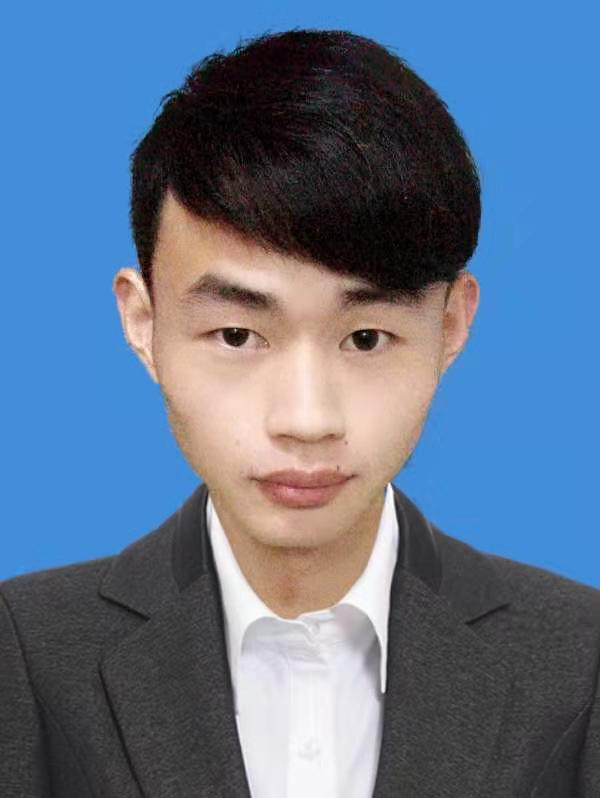
\includegraphics[width=1in,height=1.25in,clip,keepaspectratio]{photo/yongquanhu.jpg}}]{Yongquan Hu}
    received the B.S. degree from the Department of Engineering of Internet of Things at Zhejiang University of Technology, Zhejiang Province, China, in 2019. He is currently pursuing his master degree with the Department of Computer Science and Technology, East China Normal University, Shanghai, China. His current research interests are in the area of cloud computing, edge computing and machine learning techniques.
\end{IEEEbiography}

\begin{IEEEbiography}[{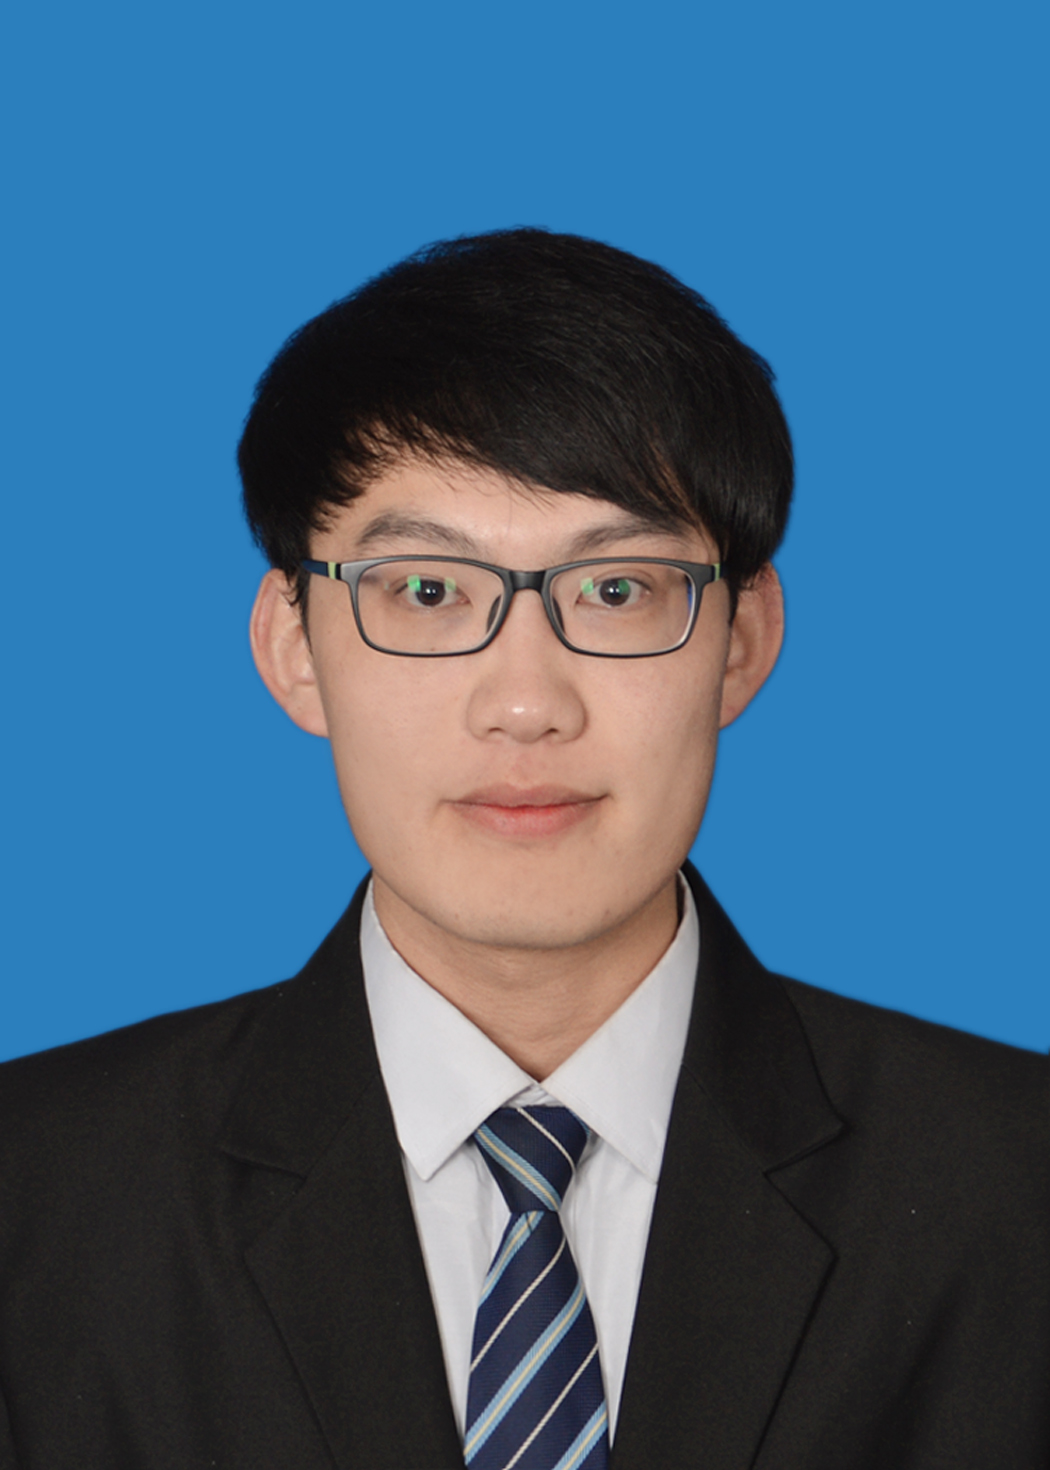
\includegraphics[width=1in,height=1.25in,clip,keepaspectratio]{photo/jiangdong.jpg}}]{Dong Jiang}
    received the B.S. degree from the Department of Electronic Information Science and Technology, Shandong University of Science and Technology, Qindao, Shandong Province, China, in 2017. He received the master degree from the Department of Computer Science and Technology, East China Normal University, Shanghai, China, in 2019. His current research interests are in computer networks.
\end{IEEEbiography}

\begin{IEEEbiography}[{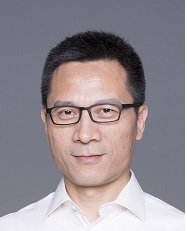
\includegraphics[width=1in,height=1.25in,clip,keepaspectratio]{photo/tongquanwei.jpg}}]{Tongquan Wei(M'11-SM'19)}
    received his Ph.D. degree in Electrical Engineering from Michigan Technological University in 2009. He is currently an Associate Professor in the Department of Computer Science and Technology at East China Normal University. His research interests are in the areas of internet of things (IoT), edge computing, cloud computing, and design automation of intelligent systems and cyber physical systems (CPS). He has published numerous papers in these areas, most of which are published in premium conferences and journals. He serves as a Regional Editor for Journal of Circuits, Systems, and Computers since 2012. He also served as the Guest Editor of the IEEE TII SS on Building Automation, Smart Homes, and Communities, the ACM TESC SS on Embedded Systems for Energy-Efficient, Reliable, and Secure Smart Homes, and the ACM TCPS SS on Human-Interaction-Aware Data Analytics for Cyber-Physical Systems. He is a senior member of the IEEE.
\end{IEEEbiography}

\begin{IEEEbiography}[{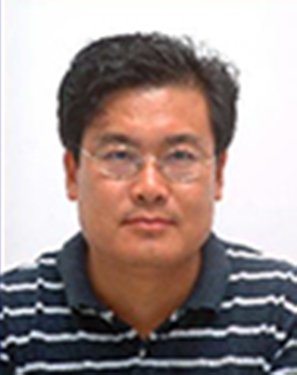
\includegraphics[width=1in,height=1.25in,clip,keepaspectratio]{photo/fukeshen.jpg}}]{Fuke Shen}
    received his Ph.D. degree in Department of Computer Science and Technology of East China Normal University in 2011. He is currently an Professor in the Department of Computer Science and Technology at East China Normal University, and director of Information Center at East China Normal University. His research interests are in the areas of computer networks communication, next generation network architecture, network protocols and their implementation, network traffic monitoring and management, and digital campus network.
\end{IEEEbiography}

\EOD

\end{document}
